\section{Introduction}

Artificial Intelligence systems in embedded and edge computing are designed to process data efficiently and make real-time decisions.
\begin{figure}[H]
    \centering
    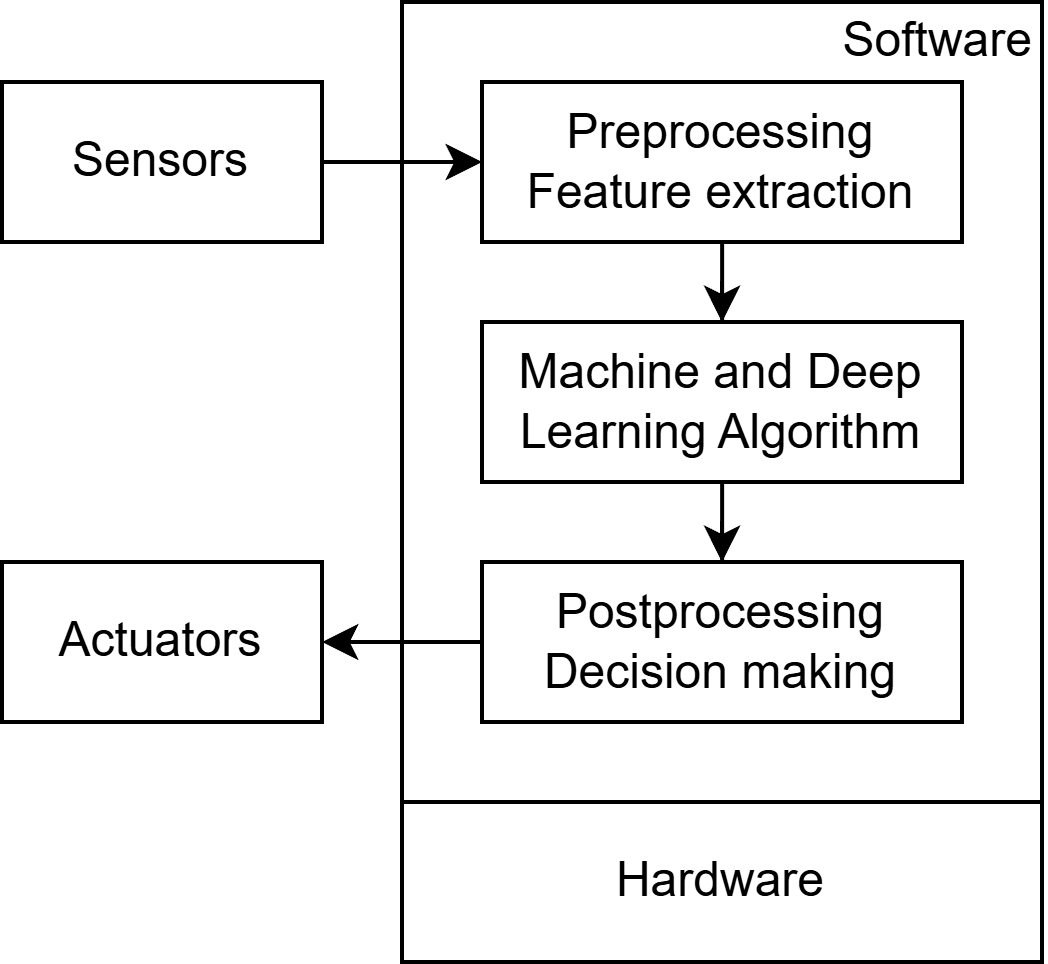
\includegraphics[width=0.5\linewidth]{images/eeai3.png}
    \caption{AI systems}
\end{figure}
The first stage is preprocessing and feature extraction, where incoming data streams from sensors are processed. 
This step involves segmenting the data into meaningful windows, removing noise, and extracting relevant features to enhance accuracy.

Once the data is preprocessed, machine learning and deep learning algorithms are applied to analyze and interpret it.
These algorithms recognize patterns, make predictions, and generate insights based on the extracted features.

Finally, in the postprocessing and decision-making stage, the system interprets the AI model's output and translates it into meaningful actions. 
This could involve making decisions, triggering automated responses, or providing feedback to users.